\chapter{Other measurements}\label{add_Meas_1}
\section{Tetrahedral array delays for a 300Hz Sine Wave}
An experiment to visualize the delays between the microphones in the tetrahedral array is conducted. In order to avoid the pressure field frequency zone of the anechoic chamber and array aliasing, 300 Hz sine wave is used. The array aperture is kept at 0.395m to approximate plane wave better. The sampling rate is 131072Hz.

\begin{figure}[H]
    \centering
    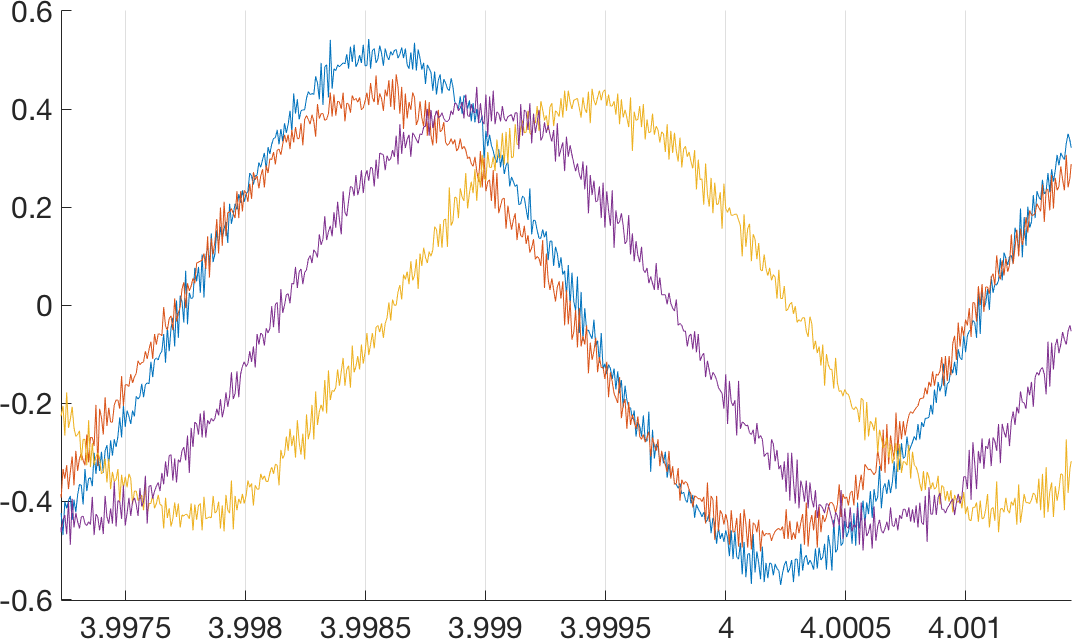
\includegraphics[width=0.8\textwidth]{Figures/delaytetra300Hz.png}
    \caption{Sine wave recorded by the four microphones}
    \label{fig:pinknoise}
\end{figure}

\begin{center}
  \begin{tabular}{ | l | c | r | r | r |}
    \hline
    Delays & Mic 1 & Mic 2 & Mic 3 & Mic 4 \\ \hline
    Mic 1 & 0 & -6&114 & 52  \\ \hline
    Mic 2 & 6  & 0 &120 & 58  \\ \hline
    Mic 3 & -114  & -120  & 0  &-61  \\ \hline
    Mic 4 & -52  & -58  &  61  & 0   \\ \hline
  \end{tabular}
  \captionof{table}{Sample delay measured between the microphones at 0 incidence (Fs= 131072Hz)}
\end{center}

Mic 1 and Mic 2 were faced towards the sound source, with Mic 3 behind and in line with the sound source. Mic 4 being the top microphone. The arrangement was such that the sound source was approximately at (90$\degree$,0$\degree$). As can be seen the delay between Mic 1 and Mic 2 is almost zero, indicating source close to 90$\degree$ azimuth. The combination of these delays can be used to predict the source direction, both in azimuth and elevation. However, if the plane wave approximation does not hold, the combination might result in a null set (No single intersection point of all the cones from the various microphone pairs).

%Variation in delay are due to the source position inaccuracies or could be due to the plane wave approximation not holding. Therefore wider peaks are to be expected and a slight shift from the zero degree position. The microphones are not calibrated in this experiment as we can see difference in amplitude are noticeable.